\newpage
\section{The RootSystem class} \label{sec:rs}

The class RootSystem is responsible for the model parameters and controls the simulation. Additionally, the class offers utility functions for post processing on a per root level, where each root is represented as a polyline, which is represented by a Python list of nodes. 

Post processing functions per segment can be found in the class SegmentAnalyser (see Section \ref{sec:sa}). A segment is a part of the root and is represented by two nodes that are connected by a straight line.



\subsection{Initialize parameters from scratch} \label{sec:from_scratch}
 
In the previous examples we opened the root system parameters from an xml file. In this example we show how to do everything in a Python script without the need of any parameter file. This is especially important if we want to modify parameters in our scripts (e.g. like it is needed for a sensitivity analysis, see Section \ref{ssec:sensitivity}).

In order to set up a simulation by hand, we have to define all relevant model parameters. This is done by creating a RootRandomParameter object for each root order or root type, and one SeedRandomParameter for each plant type. 

Note that during the simulation, the parameters for a specific root (RootSpecificParameter) are generated from the RootRandomParameter class which represents the random distributions of certain parameters.

\lstinputlisting[language=Python, caption=Example 2a]{../../examples/python/example2a_initializeparams.py}

\begin{itemize}
\item[5] Matplotlib is Python's easy way to create figures like in Matlab.\item[6] NumPy is Python's scientific computing package.

\item[9,10] Create the root type parameters of type 1 and type 2.
\item[12-38] We set up a simple root system by hand. First we define the tap root L12-L26, then the laterals L28-L38. By default all standard deviations are 0. Most parameters standard deviations can be set with an additional 's' appended to the parameter name, e.g. $lmaxs$ is the standard deviation of $lmax$, see L32
\item[40,41] Set the root type parameters.

\item[43-47] Create an object of class SeedRandomParameter which defines when basal and shoot borne roots emerge. In this example we neglect basal and shoot borne roots, and just define the seed location, and deactivate basal roots by setting their maximal number $maxB$ to 0 ($firstB$ and $delayB$ are ignored in that case). 
\item[48] Sets the root system parameters.

\item[53] We choose the simulation times in a way that we can see the temporal development, and that all lateral roots have emerged in the final time step.

\item[54-70] Within the simulation loop we create Figure \ref{fig:ip}. L58-61 defines the limits and titles. In L63 we retrieve the roots as polylines which are represented by a list of nodes. In L64-67 we plot the $x$ and $z$ coordinates for each segment ($n$, $n2$) as green line. 

\item[75-80] It is not only possible to set all model parameter, 
but to retrieve the parameters after the simulation with rs.getParameter(), which returns one value per root. For all parameters that are derived from a random distribution the root specific parameter is returned (e.g. $la$, L78), i.e. the values that were drawn from the normal distribution. The root random parameter can be accessed by adding '\_mean', '\_dev' to the parameter value (e.g. $la\_mean$, L79).

\end{itemize}

Note that all parameters can be set and modified within Python. Especially, standard deviations can be set to zero in order to be able to precisely predict the result. For example we can calculate the total root system length analytically, and check if the numerical simulation yield the (exact) same result. This is performed in the tests test\_root.py, and test\_rootsystem, which is used to test and validate CPlantBox (see folder CPlantBox/test).

With such simple simulations, we can quickly check if the model does, what we expect. For example the maximal number of laterals of above parameters is 16 
$= round(lmax - la - lb)/l_n +  1$. We can calculate the time when the final lateral emerges as $-(lmax/r)*\ln(1-(lmax-l_n/2)/lmax)$ = 122.8 days. At simulation time 125 the last lateral root that has emerged is 2.2 days old, and therefore approximately 4.4 cm long (initial growth rate $r_1 = 2$), which agrees with Figure \ref{fig:ip}.

By default the length of the apical zone is fixed, when the root is created. During growth the apical zone stays in the interval $[la - l_n/2, la+l_n/2]$. The first branch emerges at length $lb$, when the root length reaches $lb +la$.

In the following two subsections we show, how tropism parameters and inter lateral spacing will affect the resulting root system.

\begin{figure}
\centering
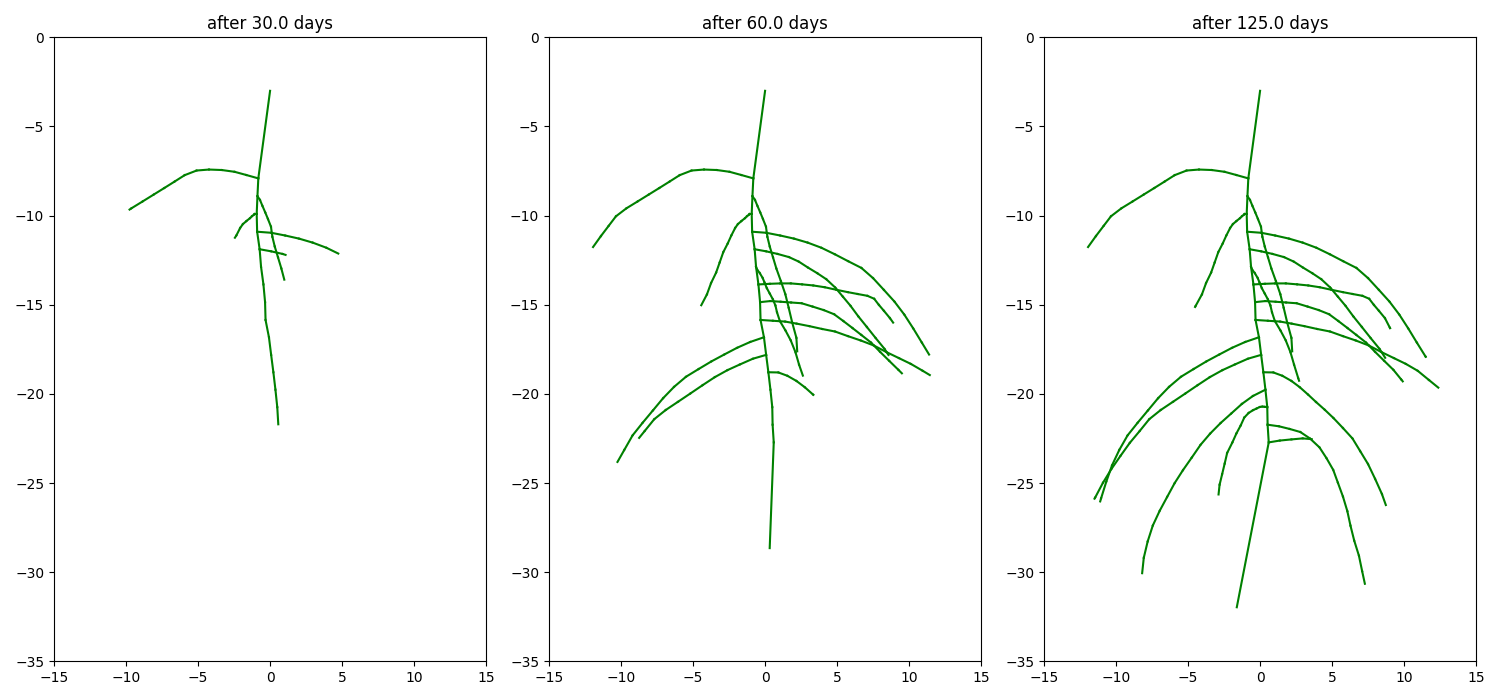
\includegraphics[width=\textwidth]{fig_initializeparams.png}
\caption{Root development} \label{fig:ip}
\end{figure}



\subsection{Root tropism parameters $N$ and $\sigma$} \label{ssec:tropism}

We show the influence of the parameters $N$ and $\sigma$ in the case of gravitropism. The parameter $N$ [1] denotes the strength of the tropism, and $\sigma$ [cm$^{-1}$] the flexibility of the root, i.e. the expected angular variation per cm root length. 

\lstinputlisting[language=Python, caption=Example 2b]{../../examples/python/example2b_tropism.py}

\begin{itemize}
\item[10-13] We choose the parameter values $N$ and $\sigma$ we want to plot. It might be interesting to change the initial insertion $angle$, and the axial resolution $dx$. Note that a change in axial resolution should not qualitatively change the resulting images.

\item[15-18] The root system is created and SeedRandomParameters are set to produce a basal root every third day. 

\item[20-23] The RootRandomParameter for tap and basal roots is defined.

\item[25-28] The loop runs over the parameters we want to modify. We create a subplot for each configuration, and start with a new root system by calling reset in L28.

\item[30-34] We set the parameters (L30,L31) and do the simulation (L33,L34)

\item[36-44] Matplotlib is used for visualization (looping over the segments is rather slow). L36 gives a list of all nodes, and L37 of all segments as two node indices. Therefore, each segment starts at node n1 and ends at node n2, as defined in L39.

\item[L48] Creates Figure \ref{fig:tropism}.
\end{itemize}

In the first column ($\sigma$=0) of Figure \ref{fig:tropism} nothing happens, because if the root has no flexibility to bend, the strength has no influence on the resulting root system. The first row ($N$=0) shows the influence of $\sigma$ only. The growth is undirected, because the strength of the gravitropism is zero. If the roots have small flexibility, they grow downwards because they initially do. 

The other subplots show different shapes of the root system. We normally derive the two parameters $N$ and $\sigma$ by visual comparison. Note that results are independent of the root axial resolution $dx$ and the temporal resolution.

\begin{figure}
\centering
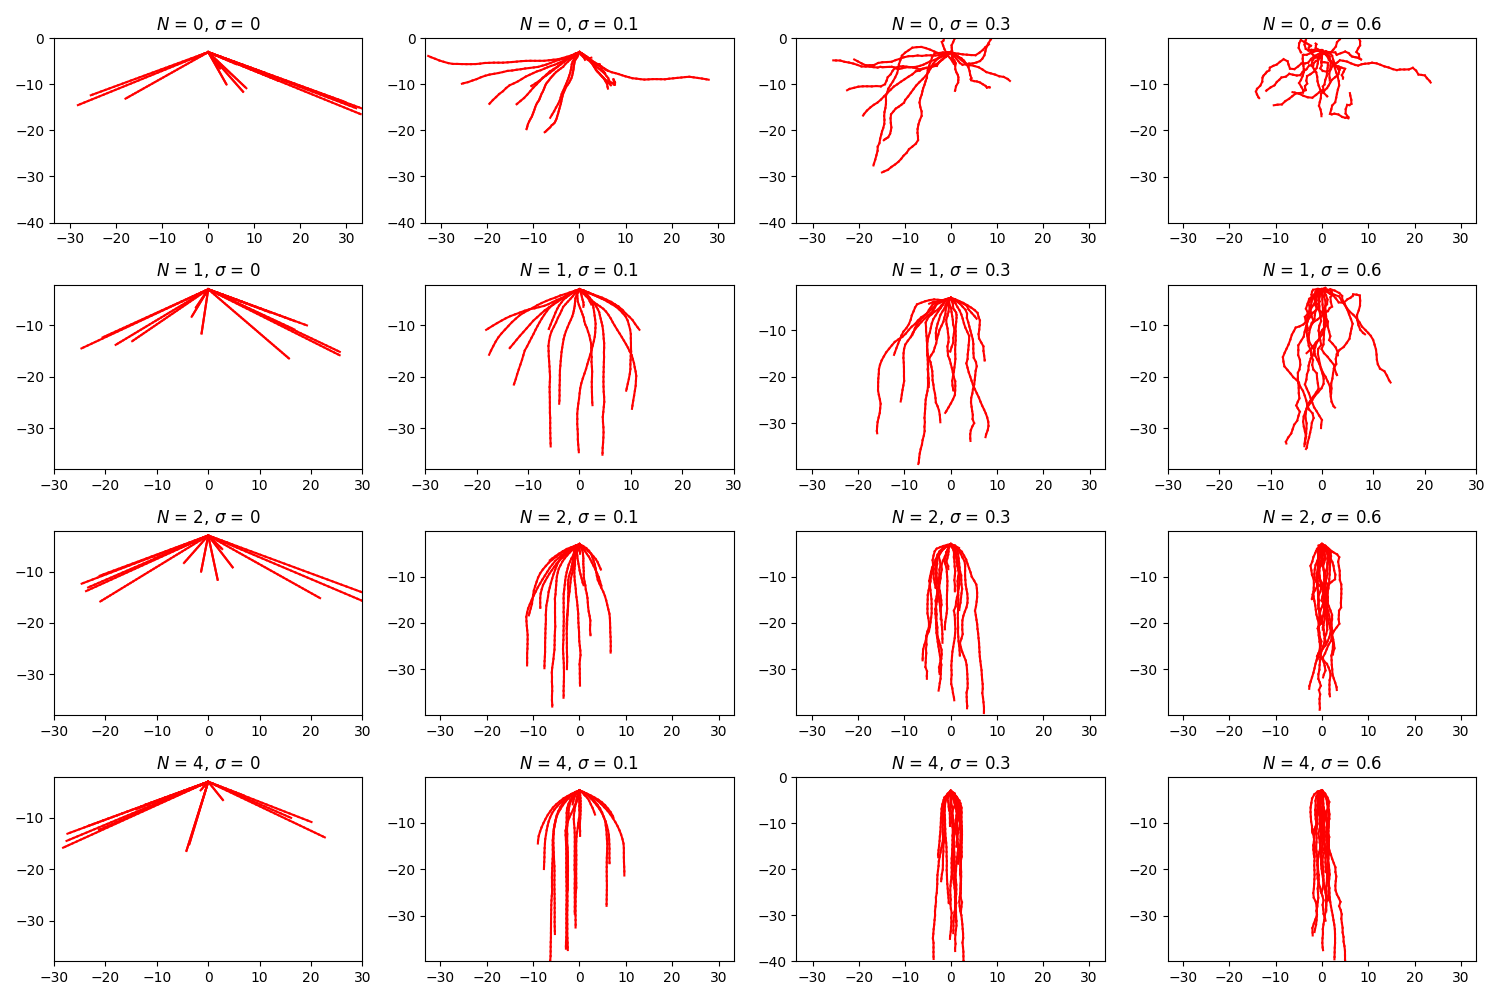
\includegraphics[width=\textwidth]{fig_gravitropism.png}
\caption{Influence of $N$ and $\sigma$ in case of gravitropism} \label{fig:tropism}
\end{figure}




\subsection{Inter lateral spacing ($ln$, $lnk$)} \label{ssec:spacing}

A single root is divided in basal zone, root branching zone, and root apical zone. Basal and apical zone are given by the parameters $la$, and $lb$ with standard deviations $la_s$ and $lb_s$. The branching zone has the size $lmax-la-lb$, where $lmax$ is the maximal root length. The branching zone is divided into inter lateral distances $l_n$, which are values drawn from a normal distribution with standard deviation $l_{ns}$. All values are fixed when the root is created This is performed in the method RootRandomParameter::realize(). The chosen parameters reflect the root growth under perfect conditions. Based on this, the root development can then be influenced by environmental conditions e.g. impeding growth speed, or lateral emergence, see Section \ref{sec:functional}.

Normally, the setting constant branching distances is sufficient, but sometime experimental data indicate that inter lateral distances are smaller, or larger near the base than near the root tip. The reason for this could be soil root interaction (e.g. root response to dense or nutritious layer), or within the genotype. We added a purely descriptive parameter to mimic such experimental observations. The parameter $lnk$, which is zero per default, defines the slope, at the mid of the branching, altering the inter lateral distance linearly along the root axis. In the following script, we demonstrate the usage of $lnk$.

\lstinputlisting[language=Python, caption=Example 2c]{../../examples/python/example2c_lateralspacing.py}

\begin{itemize}
\item[10-13] A root system with a single tap root is created. 
\item[16,16] The axial resolution, and insertion angle is defined. We take a very large axial resolution for the tap root, since we visualize the nodes later on, and we want to see only lateral branching nodes.
\item[18-24] Definition of the tap root. Standard deviations are zero, we do not want any variations. Tropism parameters are chosen in a way, that the tap root grows straight downwards.
\item[26-29] Definition of the first order lateral. Tropism is a strict exotropism (i.e. root follows its initial growth direction).
\item[31,32] The parameter values we want to visualize.
\item[36] Resets the root system (to $simTime = 0$). Root parameters are not changed. 
\item[38,39] Sets the values for this subplot. 
\item[41,42] Runs the simulation
\item[44-56] Creates the subplots. First (L47-49) we plot all segments in green. And second (L51-53) we plot all nodes of the tap root as red asterisks.
\item[58-60] Creates Figure \ref{fig:spacing}
\end{itemize}

The mid column of Figure \ref{fig:spacing} shows to different inter lateral distances, 4 (top) and 2 (cm) bot. The left column demonstrate the use of negative values for $lnk$ which results in larger distances near the base. The right column has positive values for $lnk$, which will result in smaller distances near the base. The $i$-th inter distance is calculated as $ln_i = ln + lnk (x_i-mid_x)$, where $x_i$ is the position within the branching zone, and $mid_x$ is the mid of the branching zone. This is done in RootRandomParameter::realize(). Note that $lnk$ is dimensionless and the slope in the linear equation. At mid of the branching zone the inter-lateral distance equals $ln$. 

\begin{figure}
\centering
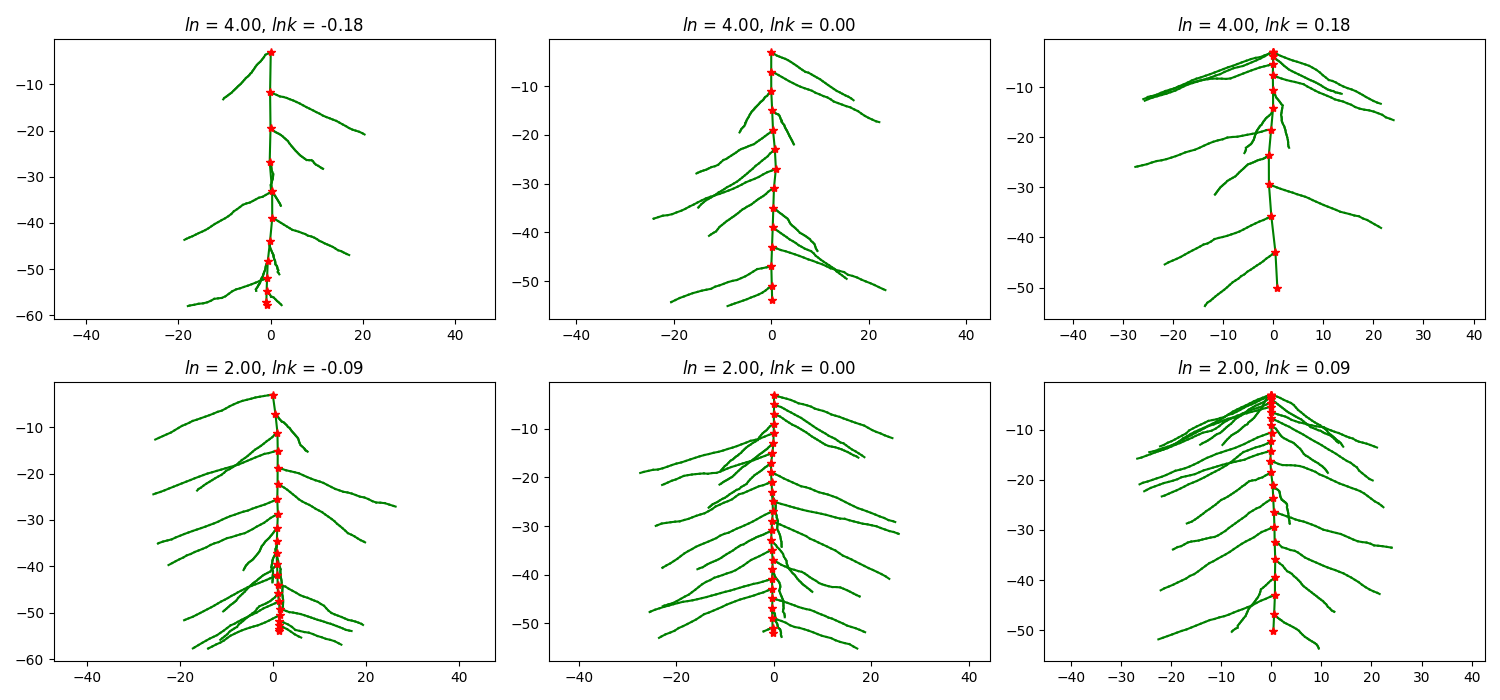
\includegraphics[width=0.99\textwidth]{fig_lateralspacing.png}
\caption{Inter-lateral spacing, larger near base (left column), constant (mid column), and smaller near base (right column) } \label{fig:spacing}
\end{figure}

In the following we show, how to analyse model results on a per root basis using the RootSystem class. To create density distributions the resulting root segments are analysed using the SegmentAnalyser class, described in Section \ref{sec:sa}.


\subsection{Root system length over time}

The following script shows how to analyse root system length versus time. 

\lstinputlisting[language=Python, caption=Example 2d]{../../examples/python/example2d_length.py}

\begin{itemize}
\item[9-14] Sets up the simulation.

\item[16-18] Defines the simulation time, time step, and the resulting number of simulate(dt) calls. 

\item[21] First we state which scalar type we want to analyse ('volume', 'surface', or 'one' would also make sense). 

\item[22] Pre-definition of the numpy arrays storing the lengths over time. 

\item[23-30] The simulation loop executes the simulation for a single time step L24. L25 calculates the type of each root (the organ subType), L26 the length (or any other parameter) of the root. L27-L30 calculates the total root length at the current time step for all roots, and for specific root types. The method rs.getParameter collects this data from the RootSystem organs. It is possible to access all root random parameters and resulting realisations using rs.getParameter. In C++ the class functions are defined in Root::getParameter, Organ::getParameter. 

\item[32-38] Creates Figure \ref{fig:length}.

\end{itemize}



\subsection{Root tips and root bases}

Next we show two options how to retrieve root tip and root base positions from a simulation:

\lstinputlisting[language=Python, caption=Example 2e]{../../examples/python/example2e_roottips.py}

\begin{itemize}

\item[14,15] Reset the simulation and simulate for only 7 days (otherwise there are so many root tips).

\item[17-18] Outputs the number of nodes and segments to get an idea how big the resulting root system is. 
Note that number of segments equals the number of nodes minus the number of base roots that will emerge. 
Base roots are tap roots, basal roots and shootborne roots.

\item[20-26] The first approach retrieves all roots as polylines L21. 
Root tips are the last nodes of the polylines L26, root bases the first nodes L25. Roots that have not started to grow have only 1 node, and are not retrieved by getPolylines().

\item[28-31] Second approach: L29 rs.getNodes() returns all nodes of the root system as a list of nodes, i.e. Vector3d objects. Each Vector3d object can be converted into a numpy array automatically, but is necessary to do that for each element of the list. The methods L30, L31 return the indices of the tips and bases. 

\item[33-41] Creates Figure \ref{fig:scatter} using the second approach.

\item[44,45] Verifies that both approaches yield the same result.

\end{itemize}

\begin{figure}
\begin{subfigure}[c]{0.5\textwidth}
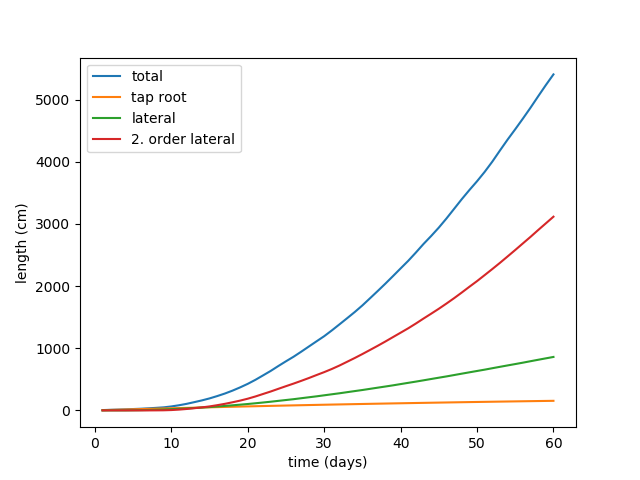
\includegraphics[width=0.99\textwidth]{example_3a.png}
\subcaption{Total root length versus time} \label{fig:length}
\end{subfigure}
\begin{subfigure}[c]{0.5\textwidth}
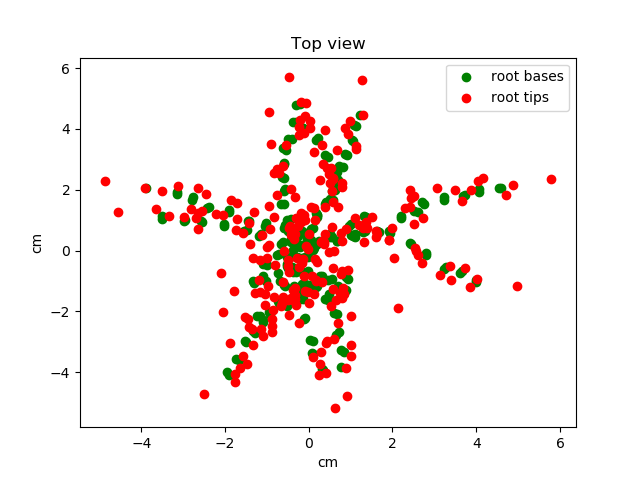
\includegraphics[width=0.99\textwidth]{example_3b.png}
\subcaption{Top view of the root tip and root bases} \label{fig:scatter}
\end{subfigure}
\caption{Root system analysis: Example 2d (a), Example 2e (b)} 
\end{figure}



\subsection{Sensitivity analysis} \label{ssec:sensitivity}

In the next part we vary given parameters in order to make a sensitivity analysis. This takes a lot of simulation runs, and we demonstrate the of use parallel computing to speed up execution.

In this exemplary sensitivity study we will vary the insertion angle of the tap and basal root, and look at the resulting change in mean root tip depth and root tip radial distance. 

\lstinputlisting[language=Python, caption=Example 2f]{../../examples/python/example2f_sensitivity.py}

\begin{itemize}

\item[12-20] Defines a function to set all standard deviations proportional to the parameter values. We use this function in the following to set the standard deviation to zero everywhere. 

\item[23-29] Parameters of the analysis. $N$ denotes the resolution of the parameter we vary, and $runs$ the number of iterations, i.e. a total of $N\cdot runs$ simulations are performed. In L29 we define the insertion angle to be varied linearly between 0 and $\pi/2$.

\item[33-52] Definition of a function that performs the simulation and returns mean root tip depth and radial distance. First we create a root system and set the standard deviation to zero L34-L36. L37, amd L39 sets the insertion angle. L41 initializes the root system and states that basal root are of root type 1 (same as tap root). The False value turns of verbosity to avoid any outputs to the console. L42 performs the simulation. L44-L51 calculates the mean root tip depth and radial distance. 

\item[55-73] This section performs the computation of all simulation runs. L55-56 preallocates the resulting arrays. L62-L68 performs the parallel computations, index $i$ is the index of the insertion angle. L71-73 calculates the mean values per simulation run.

\item[74-83] Creates the resulting Figure \ref{fig:sensitivity}. Note that the resulting curves become smoother, if the number of runs is increased (L28).

\end{itemize}

\begin{figure}
\centering
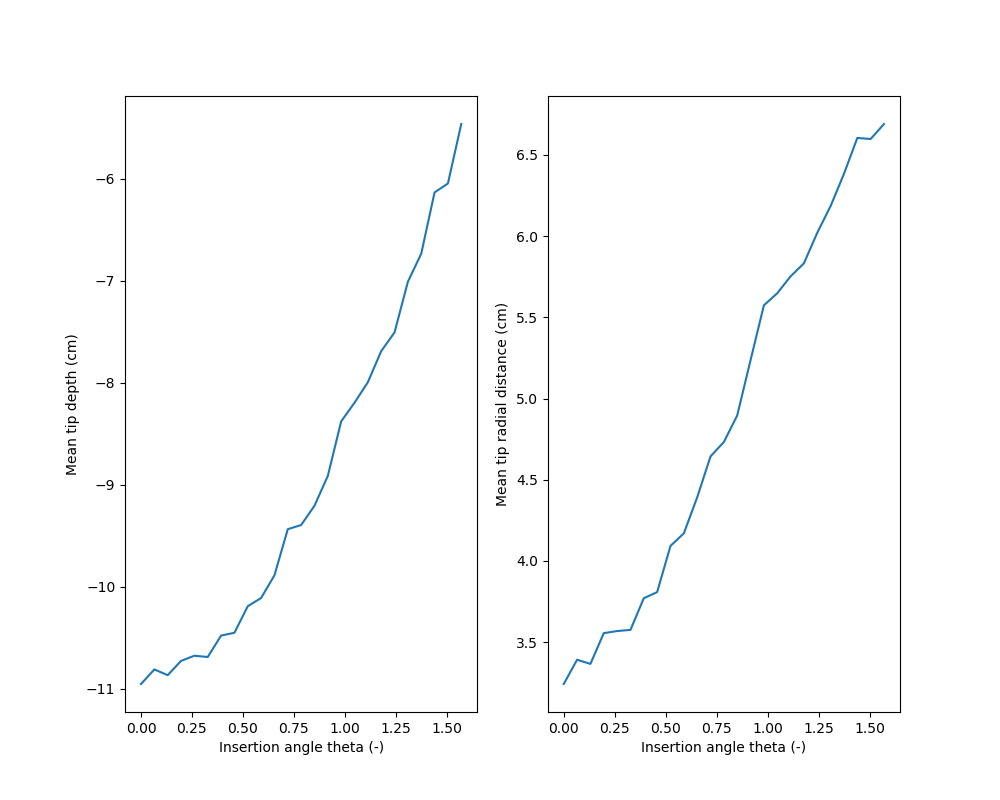
\includegraphics[width=0.7\textwidth]{example_4b.png}
\caption{Sensitivity of mean root tip depth (left) and radial distance (right) to the insertion angle theta (Example 2f) } \label{fig:sensitivity}
\end{figure}
